\documentclass[10pt]{IEEEtran}
\usepackage[utf8]{inputenc}
\usepackage{amsmath}
\usepackage{amsfonts}
\usepackage{caption}
\usepackage{graphicx}
\usepackage{amssymb}
\usepackage{cite}
\usepackage{listings}
\usepackage{url}
\renewcommand{\lstlistingname}{Configuração}% Listing -> Algorithm

\title{REDIS - RSS}
\author{Luan Bodner do Rosário \\ Felipe Veiga Ramos}
\date{\today}

\begin{document}
\maketitle

\section{Resumo}

Neste trabalho, propomos um serviço que simule o funcionamento de um \textit{RSS}, em que um determinado cliente possa se inscrever em um servidor e receber as atualizações por meio de um modelo \textit{publish/subscribe}. Esse trabalho é feito com base no servidor de estruturas de dados Redis utilizando a linguagem de programação \textit{python} em conjunto com a biblioteca que faz a interface para o Redis. Verificamos que embora a interface de programação seja aparentemente simples, a quantidade de opções e possibilidades oferecidas pelo Redis acabam sendo um problema.

\section{Introdução}
Este trabalho tem como objetivo mostrar características de baixo e alto nível da ferramenta Redis. Para atingir esse objetivo, e também explorar não só as vantagens mas também os problemas enfrentados pelos programadores e usuários que utilizam a ferramenta aqui descrita, propomos a criação de uma ferramenta um tanto quanto popular e bastante utilizada por diversos \textit{websites}.

A ferramenta que foi "recriada" em uma versão simplicada da original busca funcionar como um \textit{feed RSS}, ou seja, um programa que publica informações para um cliente inscrito para recebê-las.

Por meio deste trabalho, buscamos exemplificar características referentes à sistemas distribuídos, explorando conceitos como escalabilidade, transparência, e tratamento de falhas por meio da programação e configuração do servidor Redis.

Utilizando a linguagem de programação \textit{python}, é possível conectar APIs que fazem interface com o programa principal e fazem uso das configurações definidas pelo programador para a criação e funcionamento do servidor.

Nas próximas seções vamos explorar os conceitos estudados que explicam as ferramentas e a teoria por trás do funcionamento do programa. 

Na terceira seção, vamos discutir os conceitos de \textit{publish/subscribe}, o funcionamento geral da ferramenta Redis e buscar entender o que é e como funciona um \textit{feed RSS} genérico. Na quarta seção, vamos explorar a linguagem de programação e a biblioteca disponível para fazer interface com o Redis. Na quinta seção, vamos discutir os resultados obtidos pelos testes feitos utilizando o programa e os problemas enfrentados na tentativa de criar o serviço. 

Por fim, concluimos com o que foi possível aproveitar por meio desse experimento e o que poderia ter sido melhorado, seja pela organização do trabalho ou com relação ao programa em sí.

\section{Fundamentação Teórica}
Nesta seção, vamos explorar a teoria por trás do trabalho aqui proposto.

\subsection{\textit{RSS}}

A sigla RSS possui vários significados distintos. RSS pode significar \textit{RDF Site Summery}, ou \textit{Really Simple Syndication} e ainda \textit{Rich Site Summary}.

O RSS é um padrão desenvolvido em linguagem XML que permite que informação seja compartilhada por um determinado disseminador de dados. Portanto, RSS é um formato de entrega regular de informações, geralmente utilizado por \textit{websites} que utilizam o RSS e enviam conteúdo como um \textit{feed RSS} para quem quiser receber o conteúdo provido por um site.

RSS resolve o problema para pessoas que precisam utilizar um serviço regularmente, permitindo que um usuário seja facilmente informados resgatando as atualizações enviadas por sites no qual estejam interessados.

Como não é necessário visitar cada um dos locais você visitaria diretamente, a ferramenta permite que um usuário poupe tempo e se mantenha anônimo, não sendo necessário usar o serviço de \textit{e-mail} para receber informações.

\subsection{Redis}

Redis é um projeto de software open-source desenvolvido por Salvatore Sanfilippo, inicialmente pela VMWare e por fim sendo desenvolvida por Redis Labs. O lançamento inicial da ferramenta foi em dez de abril de 2009.

A ferramenta Redis é comumente referida como um servidor de estrutura de dados. Isso significa que a feramenta da acesso à uma série de estruturas de dados mutáveis a partir de uma lista de comandos, enviadas por meio de um modelo cliente-servidor utilizando sockets TCP e um protocolo simples.

O modelo cliente servidor é uma estrutura de aplicação distribuída que compartilha as tarefas e cargas de trabalho entre os fornecedores de um recurso ou serviço, desiginados como servidores e os requerentes dos serviços.

Na distribuição Redis, uma máquina serve como servidor das estruturas de dados e as outras máquinas da rede podem se conectar e acessar os dados armazenados e os comandos disponíveis, desta forma, diferentes processos podem enviar e modificar dados de forma compartilhada.


\begin{figure}
	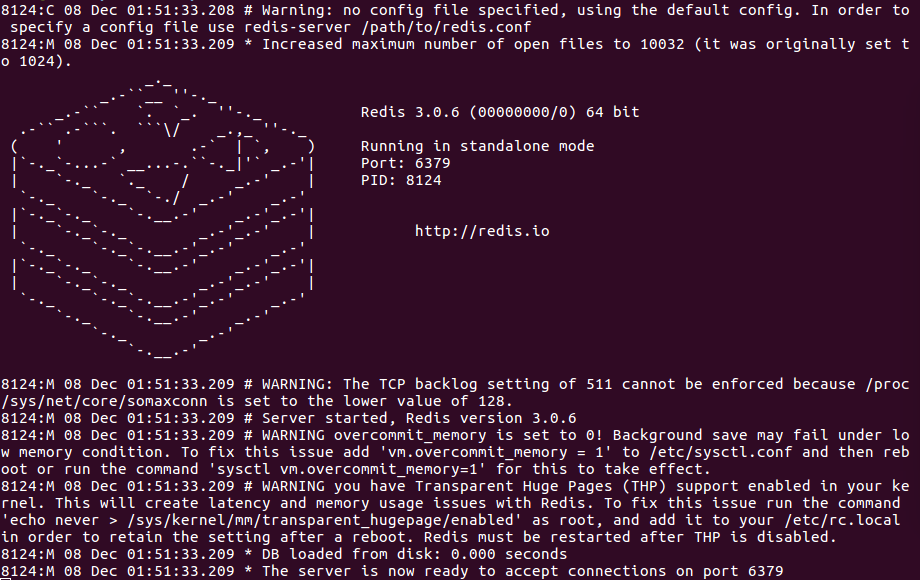
\includegraphics[scale=0.35]{server.png}
	\label{fig:server}
    \caption{Exemplo de um servidor Redis}
\end{figure}

Entre as estruturas suportadas pelo Redis temos:
\begin{itemize}
\item \textit{Strings}
\item \textit{Hashes}
\item \textit{Sets} e \textit{Sorted Sets}
\end{itemize}

As estruturas implementadas no Redis possuem algumas propriedas especiais:
\begin{itemize}
\item Armazenamento em disco, mesmo que elas estejam modificadas e armazenadas no servidor. Desta forma, REDIS é capaz de manter sua eficiencia.
Redis oferece opções comuns em banco de dados, como replicação, níveis de durabilidade mutáveis , etc.

\item A implementação de estruturas de dados geram \textit{stress} na memória, então, as estruturas de dados dentro do Redis provavelmente vai utilizar menos memória que as mesmas estruturas de dados dentro de linguagens de programação de alto nível.
\end{itemize}

Outra forma de se analizar o Redis é enchergá-lo como uma versão mais complexa de memchaced, onde as operações são apenas SET e GET. Redis no caso, possui dados mais complexos e mais operações possíveis também.

Várias linguagens possuem APIs dando suporte para Redis, incluindo: ActionScript, C, C++, C\#, Chicken Scheme, Clojure, Common Lisp, D, Dart, Erlang, Go, Haskell, Haxe, Io, Java, JavaScript (Node.js), Julia, Lua, Objective-C, OCaml, Perl, PHP, Pure Data, Python, R, Racket, Ruby, Rust, Scala, Smalltalk and Tcl.

Além disso, o Redis é utilizado por diversas companias muito conhecidas, como \textit{Twitter, GitHub, Weibo, Pinterest, Snapchat, Craigslist, Digg, StackOverflow} e \textit{Flickr}

\subsection{\textit{Publish/Subscribe}}

O modelo \textit{publish/subscribe} é um padrão de mensagens onde um remetente, chamado \textit{publisher} não programa as mensagens para serem enviadas para destinatários específicos, mas sim para canais de mensagem. Os destinatários, chamado \textit{subscribers} se inscrevem em determinado canal para receberem as mensagens.

Em vários sistemas \textit{publish/subscribe}, os remetentes mandam as mensagens para um \textit{broker}, que realiza a filtragem de mensagens.

Neste modelo, os remetentes não tem conhecimento dos inscritos, ou se ao menos eles existem. Desta forma, ambas as partes do modelo podem permanecer ignorantes da topologia do sistema, podendo dar continuidade às suas operações de maneira independente.

\subsubsection{\textit{Publish/Subscribe} no Redis}

As funções \textit{SUBSCRIBE}, \textit{UNSUBSCRIBE} e \textit{PUBLISH} são responsáveis pela implementação do paradigma \textit{Publish/Subscribe}. Por Exemplo, para se inscrever a um canal foo e bar, o cliente manda um comando \textit{SUBSCRIBE} dando o nome para os canais:
\begin{lstlisting}
SUBSCRIBE foo bar
\end{lstlisting}

Mensagens eviadas por outros clientes para esses canais serão enviados pelo Redis para todos os clientes inscritos.
Um cliente inscrito por um ou mais canais não devem enviar comandos, apesar de poderem se inscrever e cancelar a inscrição em outros canais. As respostas para estes comandos são enviados em forma de mensagens, para que o cliente possa ler as mensagens de forma coerente, o primeiro elemento da mensagem indica o tipo.

Formato das mensagens enviadas são:
\begin{itemize}
\item \textit{Subscribe} : significa que a inscrição ocorreu com sucesso dado pelo segundo elemento da mensagem. O terceiro elemento representa o numero de canais em que você está inscrito.
\item \textit{Unsubscribe} : significa que o cancelamento da inscrição ocorreu com sucesso dado pelo segundo elemento da mensagem. O terceiro elemento representa o numero de canais em que você está inscrito.
\item \textit{Message} : é a mensagem recebida como resultado de um comando \textit{PUBLISH} enviado por outro cliente. O segundo elemento é o nome do canal enviado, e o terceiro é a mensagem.  
\end{itemize}

\subsection{Redis Sentinel}

O \textit{Redis Sentinel} possibilita a disponibilidade do servidor Redis. Em termos práticos, significa que usando o \textit{Sentinel} pode criar resistência do servidor mesmo sem intervenção humana.

Essa sentinela também é capaz de cumprir outras tarefas como monitoramento, notificação e funciona como um provedor de configuração para os clientes.

A lista de capacidade do sentinela é definida:
\begin{itemize}
\item Monitoração: O sentinela constantemente checa se as instancias do Redis estão funcionando normalmente.
\item Notificação: A sentinela notifica o administrador do sistema, outros programas, a partir de uma API, que alguma coisa está errada com o Redis.
\item Recuperação: Se um mestre não está funcionando, a sentinela pode começar um processo de tornar um escravo para promove-lo para um mestre, reconfigurando os outros escravos para utilizar o novo mestre.
\item Configurador: A sentinela é um serviço de autoridade para os clientes, sendo que eles se conectam com a sentinela para perguntar o endereço do novo mestre.
\end{itemize}

O \textit{Redis Sentinel} é um sistema distribuído, ja que diversos processos estão cooperando entre sí com base na configuração dada dentro do sentinela,além disso, o \textit{Redis Sentinela} deve rodar em conjunto com o servidor Redis.

\section{Materiais e Métodos}
Nesta seção, serão descritos os detalhes de implementação na linguagem escolhida, a configuração do servidor Redis e a configuração do \textit{Redis Sentinel}.

\subsection{Redis .conf}

O servidor Redis necessita de certas configurações que habilitem o seu funcionamento da maneira esperada para que determinada tarefa seja completada. Na distribuição Redis, o arquivo redis.conf possui as configurações padrões para o funcionamento do Redis.

Neste arquivo foram feitas as configurações necessárias para que o Redis funcione no contexto de uma ferramenta de RSS.

\subsubsection{Bind}

O \textit{bind} oferece a interface na qual o Redis escuta por conexões, o valor padrão do \textit{bind} é dado pela linha a seguir:

\begin{lstlisting}[caption=Diretiva de conexão]
#bind 127.0.0.1
\end{lstlisting}

Inicialmente não comentada, essa diretiva força o Redis a escutar apenas o endereço \textit{IPv4 lookback}, ou seja, só aceitará conexões a partir do computador no qual o servidor está rodando.

O servidor Redis no caso do RSS tem o \textit{bind} comentado, significando que o Redis vai continuar escutando para qualquer cliente que queira se conectar.

\subsubsection{Protected Mode}

O modo de proteção é uma camada de proteção para impedir que instâncias do Redis que permaneceram abertas na internet sejam acessada e exploradas.

Se nenhuma senha foi configurada e o servidor não especifica o IP pela diretiva \textit{bind}, dado que o modo de proteção esteja ligado, então o servidor só vai aceitar conexões a partir do endereço de \textit{loopback}.

No servidor Redis para o RSS, o modo de proteção está desligado, para que os clientes não precisem de autenticação para se conectar.

\begin{lstlisting}[caption=Diretiva de proteção]
protected-mode no
\end{lstlisting}

\subsubsection{Replicação}

A replicação se refere a forma m que os dados são copiados do mestre para o escravo. A replicação é automática e não precisa de intervenção do cliente.

Quando um escravo perde conexão com o mestre, ou quando a replicação está em progresso, o escravo vai responder com uma mensagem de erro, impedindo a execução de qualquer comando.

\begin{lstlisting}[caption=Diretiva de replicação]
slave-serve-stale-data yes
\end{lstlisting}

Além disso, é possível definir se um escravo é capaz de escrever e mandar dados para o servidor, caso essa opção seja desabilitada, o cliente só pode ler informações já existentes.

\begin{lstlisting}[caption=Diretiva de leitura]
slave-read-only yes
\end{lstlisting}

\subsection{Redis Sentinel .conf}

O programa sentinela também possui um arquivo de configuração, parcialmente definido pelo programador e parcialmente escrito em tempo de execução.

O programa sentinela precisa de no mínimo três instâncias em execução para que o funcionamento do servidor Redis seja analisado de forma robusta.

Uma das possíveis configurações na sentinela é o monitoramento do mestre. É viável determinar qual é o endereço do mestre que deve ser monitorado, e caso o servidor saia de serviço, o sentinela promove um escravo e modifica o artigo de configuração.

Neste caso, verificamos o servidor presente neste mesmo computador:
\begin{lstlisting}
sentinel monitor mymaster 127.0.0.1 6379 2
\end{lstlisting}

Para este trabalho, esta é a principal função do sentinela: manter o serviço de RSS em funcionamento mesmo que o servidor inicial não esteja mais em funcionamento.


\subsection{O programa}

O programa que simula um RSS simplificado foi feito utilizando a linguagem \textit{python} por meio da interface \textit{python redis}, que cria um \textit{wrapper} para a utilização dos comandos presentes no Redis.

No arquivo \textit{ps.py}, as classes estão divididas da seguinte maneira:
\begin{itemize}
\item \textit{Class Listener}: Esta é a classe que faz uso da interface com o Redis para fazer as operações de inscrição e cancelamento de inscrição. Também é utilizada para mostrar e tratar as mensagens recebidas, já que por meio de uma \textit{thread}, fica esperando mensagens chegarem no canal.

\begin{lstlisting}[language=Python, caption=Classe \textit{Listener}]
class Listener(threading.Thread):
    def subscribe(self, canal)...
    def unsubscribe(self)...
    def imprime_mensagem(self, item) ...
    def run(self)...
\end{lstlisting}

\item Outros métodos: Os outros métodos dentro do programa utilizam a classe \textit{Listener} para chamar as devidas funções do Redis e também lendo as entradas providas pelo usuário.
Por exemplo: 
\begin{lstlisting}[language=Python, caption=Método de Inscrição]
def inscrever(pubsub):
    canal = input("Nome do canal:")
    l = Listener(pubsub,canal)
    l.start()
    return canal,l
\end{lstlisting}

Como citado, o método de inscrição utiliza o \textit{Listener} e uma entrada do usuário, dando início a \textit{thread} que fica escutando por novas mensagens.

\item Interface básica: Para fazer interface com o usuário, utiliza-se a própria linha de comando, pedindo as entradas necessárias para o funcionamento do programa.

Essas entradas estão no formato numérico, mostrando as determinadas possibilidades dentro do sistema.

\begin{lstlisting}[language=Python, caption=Interface]
//Cancelar inscricoes
option = int(input("Digite a opcao:"))
if option == 0:
   finalizar(inscritos)
\end{lstlisting}

\end{itemize}

\section{Resultados e Discusões}

Nesta seção, apresentamos o que foi aprendido durante o desenvolvimento desta ferramenta básica que funciona de forma similar à um \textit{feed RSS}.

\subsection{Resultados}

Por meio dessa implementação, observamos que a ferramenta Redis é extremamente flexível e a variedade de aplicações que podem ser produzidas utilizando-a como base é extremamente grande.

Além das possibilidades criadas pela interface para linguagens de programação (neste caso, para a linguagem \textit{python}), temos também os arquivos de configuração que podem alterar completamente o sistema aqui proposto.

Essa característica do Redis é também um problema para um programador não experiente com a ferramenta. A quantidade de mudanças e condições que devem ser levadas em consideração para o funcionamento do Redis de a acordo com o problema a ser resolvido.

Para um usuário, ou para um desenvolvedor que não conhece as possibilidades e as aplicações do Redis, a interface para linguagens de programação podem aparentar ser extremamente simples e fácil de utilizar, o que não é necessariamente verdade. A interface para a linguagem C é, em exemplos básicos, extremamente simples, mas quando a complexidade do programa a ser desenvolvido aumenta, a interface também se torna mais obscura e problemática. Esse problema foi a principal razão de utilizar a linguagem \textit{python}.

O máximo que podemos afirmar por meio deste experimento é que a possibilidade de implementação de um RSS completo é possível e a parte de configuração do servidor Redis e suas sentinelas é definitivamente a que requer mais tempo e recursos para ser completada.

Outro resultado dessa implementação é o aprendizado da base do funcionamento do Redis e como lidar com segurança e persistência devem ser prioridade para o programador.

Infelizmente, o experimento não foi completo, ja que por restrições de tempo, não foi possível implementar e testar um sistema completo em funcionamento, o que traria ainda mais informações e aprendizado para os desenvolvedores.

Apesar disso, os conceitos de RSS podem ser exemplificados por esse programa, que mesmo incompleto, é funcional para o envio e recebimento de mensagens por meio do modelo \textit{publish/subscribe}.

\subsection{Discussão}

Como citado anteriormente, não foi possível implementar um programa completo com o escopo projetado e discutido nos capítulos iniciais. Apenas um programa simples que exemplifica os conceitos relativamente mais básicos da teoria apresentada e discutida nas seções anteriores.

Por fim, outros pontos importantes discutir, além da dificuldade de configuração do servidor, temos:

\begin{itemize}
\item Problemas de implementação: O programa desenvolvido não é completamente seguro. Devido à falta de tempo, não foi possível fazer toda o tratamento de exceção necessário para garantir o funcionamento perfeito RSS simplificado.
\item Persistência: Não foi possível configurar o servidor de forma que as mensagens enviadas para os canais de comunicação persistam para os clientes.
\item Criação de canais: A criação de canais e gerenciamento tiveram que ser modificados da idéia original. Nesta versão, os canais são criados em tempo de execução, sendo possível gerenciar os canais em que um usuário está escrito, e como citado acima, não existe persistência do canal.
\item Facilidade de Programação: A interface do Redis para a linguagem \textit{python} é bastante simples. Apesar de extremamente simplificado, a interface e a linguagem facilitaram a implementação.
\end{itemize}

\section{Conclusões}

A partir deste trabalho, podemos concluir que a ferramenta Redis é versátil e dá suporte para diversos tipos de aplicação que podem ser implementadas utilizando as principais linguagens do mercado.

Apesar da flexibilidade, a configuração do servidor é um tanto quanto complexa devido a abertura do sistema para o programador. Portanto, o foco durante o desenvolvimento de um serviço baseado no Redis deve ser em cima primeiramente da configuração do Redis e de suas sentinelas.

\nocite{*}
\bibliographystyle{ieeetr}  

\bibliography{Ref}


\end{document}